\documentclass[11pt]{book}
\usepackage[bottom=2cm,
  top=3cm, left=3cm, right=2cm]{geometry}
\usepackage{graphicx}
\usepackage[italian]{babel}
\usepackage{float}
\usepackage{hyperref}
\setlength{\parindent}{0pt}
\setcounter{chapter}{1}

\begin{document}

\chapter{Il DMA Controller}

Prima di affrontare la trattazione, specifichiamo che prenderemo in
esame il \textbf{DMAC} realizzato dal componente \textbf{i8237A}.

\textbf{DMA} sta per \textbf{Direct Memory Access} ed \`e una
modalit\`a di I/O che viene utilizzata in sistemi
\textbf{multimaster}. Con il DMA la CPU viene sollevata dall'incarico
di interagire con le interfacce di I/O e demanda queste operazioni ad
un altro componente che \`e il DMA Controller (DMAC). La CPU ed il
DMAC si \textit{accordano} sul passaggio di testimone tramite il
protocollo {\tt HOLD/HOLDA}. Quando il DMAC richiede il controllo, la
CPU rilascia il bus dati che potr\`a quindi essere usato dal DMAC.

Un esempio di queste operazioni \`e il trasferimento di informazioni
da memoria esterna a memoria principale. Il DMAC assume il controllo
ed effettua il trasferimento. La CPU rilascia soltanto il bus dati ma
pu\`o continuare a svolgere le operazioni che non richiedano accesso
al bus. Senza il DMAC la CPU avrebbe dovuto gestire gli interrupt
relativi e sospendersi ogni volta per gestire le richieste delle
periferiche.

Come la CPU, anche il DMAC \`e in grado di generare indirizzi, dati e
segnali di controllo per effettuare trasferimenti di dati fra memoria
e dispositivi di I/O.

\section{Modalit\`a di trasferimento}

Il trasferimento tra DMA e I/O pu\`o avvenire in diversi modi: 
\begin{itemize}
\item \textbf{burst}: una volta iniziato il trasferimento, il DMAC
  mantiene il controllo del bus finch\'e non \`e terminato a discapito
  della CPU; 

\item \textbf{cycle stealing}: il DMA esegue il trasferimento di
  parole un solo ciclo completo alla volta (cio\`e per ogni ciclo si
  interfaccia con la periferica ed esegue il trasferimento solo se \`e
  pronta, in altre parole effettuando un \textit{handshaking}). Come
  risultato il tempo nel quale la CPU \`e bloccata \`e pi\`u
  frammentato.

\end{itemize}

Sebbene vi siano quattro canali, solo un trasferimento pu\`o essere
attivo per volta.

Ecco ad esempio come si pu\`o svolgere un trasferimento da memoria a
periferica di I/O o viceversa: 

\begin{enumerate}
\item Quando una periferica deve effettuare un trasferimento invia il
  segnale \texttt{DRQi} al DMAC;

\item Il DMAC verifica se ci sono altri trasferimenti pi\`u prioritari
  ed in caso contrario richiede tramite il segnale \texttt{HOLD} alla
  CPU il controllo del bus. Il segnale \texttt{HOLD} non pu\`o essere inibito.

\item La CPU termina il ciclo sul bus ed attiva il segnale
  \texttt{HOLDA} per garantire al DMAC il controllo del bus. Questo
  segnale si attiva dopo che la CPU ha messo tristate il bus dati, il
  bus degli indirizzi, il bus dei comandi ed i segnali
  \texttt{M/IO\#}, \texttt{W/R\#}, \texttt{D/C\#} e \texttt{CACHE\#}.

\item A questo punto il DMAC prende il controllo e genera un indirizzo
  per la memoria ed il segnale \texttt{DACKi} (un segnale di
  acknowledgment) verso l'interfaccia che ha richiesto il
  trasferimento.

\item A seconda che il trasferimento sia da memoria a interfaccia o da
  interfaccia a memoria genera la coppia di segnali \texttt{MEMRD\#} -
  \texttt{IOWR\#} oppure \texttt{IORD\#} - \texttt{MEMWR\#}. \`E
  adesso che il trasferimento pu\`o aver luogo. Quando termina,
  l'interfaccia disabilita il segnale \texttt{DRQi} ed il DMAC
  rilascia il bus disabilitando il segnale \texttt{HOLD}. Il
  processore disabiliter\`a di conseguenza il segnale \texttt{HOLDA}.

\end{enumerate}

In DMA si possono fare trasferimenti \textbf{Fly-by} e trasferimenti
\textbf{Flow-through}: questi ultimi sono trasferimenti di dati che
prevedono il passaggio attraverso il DMAC, mentre gli altri sono al
volo, da periferica a memoria o viceversa senza passaggio dal DMAC. I
trasferimenti fly-by possono essere utilizzati per trasferire dati da
una periferica alla memoria o viceversa, ma non fra due periferiche o
fra due aree di memoria perch\'e non potrebbero essere indirizzate
contemporaneamente.


\subsection{Modalit\`a di trasferimento singolo}

Approfondiamo quanto succede dal passo 4 della sequenza
precedentemente indicata. Il DMAC svolge le seguenti operazioni:

\begin{enumerate}
\item fornisce sul bus degli indirizzi l'indirizzo della locazione di
  memoria in cui verr\`a letto o scritto il dato;
\item attiva la coppia di segnali di lettura dalla memoria e scrittura
  sul dispositivo o quella di lettura dal dispositivo e scrittura in
  memoria;
\item attiva il segnale di \texttt{DACK} a fronte del quale la
  periferica disattiva il \texttt{DREQ};
\item decrementa il contatore del numero di parole da trasferire
  (vedremo in seguito in quale registro \`e contenuto);
\item aggiorna il puntatore alla locazione di memoria da cui leggere o
  su cui scrivere e disasserisce \texttt{HOLD} a seguito del quale la
  CPU disattiva \texttt{HOLDA}.
\end{enumerate}

Il DMAC tiene il controllo del bus per il tempo necessario ad
effettuare una lettura o una scrittura, cio\`e pochi cicli di
clock. In questo intervallo di tempo \`e come se la CPU non ricevesse
il clock. \`E per questo che si parla di \textbf{cycle
  stealing}. Ovviamente nel momento in cui si debbano trasferire pi\`u
dati, si devono svolgere pi\`u volte i passi illustrati.

\subsection{Modalit\`a di trasferimento burst}

La modalit\`a burst, o \textit{a blocchi}, differisce dalla precedente
solo in quanto il segnale \texttt{HOLDA} viene disasserito soltanto
nel momento in cui diventa 0 il contatore dei dati rimasti da
trasferire. La CPU risulta esclusa dall'uso del bus per tutta la
durata del trasferimento.

\section{Modalit\`a di funzionamento di un canale}

\begin{itemize}
\item \textbf{Single Transfer Mode}: \`e la modalit\`a di
  trasferimento singolo illustrata prima.

\item \textbf{Block Mode}: \`e la modalit\`a burst illustrata in
  precedenza.

\item \textbf{Demand Mode}: a fronte di una richiesta attiva il DMAC
  si impossessa del bus e continua ad eseguire trasferimenti fino a
  che la richiesta non si disattiva. Al disattivarsi della richiesta
  rilascia il bus (modalit\`a tipicamente burst). Continua a
  trasferire fino a che il \texttt{DREQi} rimane attivo.

\item \textbf{Cascade Mode}: ai pin \texttt{DREQi} e \texttt{DACKi}
  vengono collegati i pin \texttt{HOLD} e \texttt{HOLDA} di un altro
  DMA controller per implementare una cascata di DMAC ed aumentare il
  numero di periferiche gestibili tramite DMA.
\end{itemize}

\section{Piedini del DMAC}

Possiamo osservare in figura \ref{dmac} la struttura del DMAC.

\begin{figure}[h!]
  \centering
  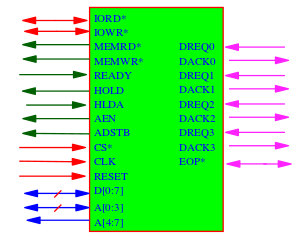
\includegraphics[width=.5\textwidth]{images/dmac.png}
  \caption{Il DMA Controller}
  \label{dmac}
\end{figure}

I segnali che vediamo sono:
\begin{itemize}
\item {\tt IORD\#}: viene attivato nel momento in cui si deve leggere
  da una periferica di I/O. Il cancelletto indica che il segnale \`e
  attivo basso.
\item {\tt IOWR\#}: si attiva quando si deve scrivere su una
  periferica di I/O.
\item {\tt MEMRD\#}: attivo quando bisogna leggere dalla memoria.
\item {\tt MEMWR\#}: come si pu\`o immaginare viene attivato nel
  momento in cui bisogna scrivere sulla memoria.
\item {\tt READY}: \`e un segnale in ingresso al DMAC e viene
  utilizzato da una periferica per segnalare quando \`e pronta per
  trasferire un nuovo dato. \`E solo allora che il DMAC abilita il
  trasferimento per non tenere bloccato inutilmente il bus che invece
  potrebbe essere utilizzato dalla CPU.
\item {\tt HOLD}: come abbiamo visto prima \`e un segnale comandato
  dal DMAC, dunque in uscita da esso, e serve a richiedere il
  controllo del bus.
\item {\tt HOLDA}: \`e un segnale in entrata, comandato dalla CPU, che
  conferisce al DMAC il ruolo di master.
\item {\tt AEN}: viene utilizzato per prendere il controllo del bus
  degli indirizzi.
\item {\tt ADSTB}: sta per Address Strobe e quando \`e attivo fa si
  che i bit \item {\tt D[0:7]} vengano usati per indirizzamento,
  affiancando i bit \item {\tt A[0:7]}. Viene spiegato meglio nel
  seguito.
\item {\tt CS\#}: \`e il chip select.
\item {\tt CLK}: \`e il clock.
\item {\tt RESET}: non ha bisogno di spiegazioni.
\item {\tt D[0:7]}: sono 8 bit dedicati al trasferimento di dati.
\item {\tt A[0:3]}: sono 4 collegamenti bidirezionali che possono
  essere usati o dal DMAC per formare quattro dei bit di
  indirizzamento oppure sono ingressi per il DMAC che selezionano il
  registro interno da leggere.
\item {\tt A[4:7]}: questi sono altri quattro bit usati per
  l'indirizzamento, ma al contrario dei precedenti sono segnali
  unidirezionali generati dal DMAC.
\item {\tt DREQi}: \`e il segnale tramite cui una periferica richiede
  un trasferimento dati. L'indice i varia da 0 a 3 dato che il DMAC
  gestisce 4 canali. Dev'essere mantenuto attivo fino a che il DMAC
  non attiva \item {\tt DACKi}.
\item {\tt DACKi}: il DMAC notifica alla periferica tramite questi
  segnali l'avvio di un trasferimento sul canale \textit{i}.
\item {\tt EOP\#}: sta per \textit{End Of Process}, \`e attivo basso e
  viene utilizzato dal DMAC per notificare la fine della sua
  elaborazione. {\tt EOP\#} \`e per\`o anche un ingresso e pu\`o
  essere usato per forzare l'arresto dell'operazione di trasferimento
  in corso.
\end{itemize}

Viene spontanea una domanda: se per indirizzare la memoria si
utilizzano anche i piedini \texttt{D[7..0]}, i dati dove passano? Il
DMAC asserisce il comando \texttt{ADSTB} che fa si che gli 8 bit di
indirizzo forniti da \texttt{D[7..0]} vengano memorizzati in un latch
esterno e subito dopo quest'operazione, il segnale \texttt{AEN} fa in
modo da abilitare l'uscita del latch verso il bus degli
indirizzi. L'uso dei bit \texttt{D[7..0]} per l'invio di dati diventa
quindi nuovamente possibile. Vedremo pi\`u avanti come ottenere gli
altri 16 bit mancanti per arrivare a 32.

\

\section{I registri interni al DMAC}

Analizziamo ora i registri interni al DMAC.

\subsection{Command Register}

\`E un registro i cui 8 bit sono dedicati alla \textbf{configurazione
  globale del DMAC}. Gli 8 bit sono:

\begin{enumerate}
\setcounter{enumi}{-1}
\item \texttt{Memory-To-Memory Enable}
\item \texttt{Channel 0 Hold Address Enable}
\item \texttt{Controller Enable*}
\item \texttt{Compressed Timing Enable}
\item \texttt{Fixed/Rot. Priority} (0/1)
\item \texttt{Late/Ext. Write} (0/1)
\item \texttt{DREQ HI/LO} (0/1)
\item \texttt{DACK HI/LO} (0/1)
\end{enumerate}

\subsection{Mode Register}

Anche questo registro \`e di 8 bit e viene utilizzato per specificare
i \textbf{parametri specifici di ciascun canale}.

\begin{itemize}
\item I bit 0 e 1 selezionano il canale (avendo quattro canali servono
  due bit);
\item I bit 2 e 3 impostano l'operazione:
  \begin{itemize}
  \item \texttt{00}: verify
  \item \texttt{01}: write to mem
  \item \texttt{10}: read from mem
  \item \texttt{11}: illegale
  \item \texttt{XX}: se cascade mode
  \end{itemize}
\item il bit 4 abilita (1) o disabilita (0) l'autoinizializzazione del
  canale;
\item il bit 5 abilita l'incremento (0) il decremento (1) degli
  indirizzi;
\item i bit 6 e 7 impostano la modalit\`a:
\begin{itemize}
\item \texttt{00}: Demand
\item \texttt{01}: Single
\item \texttt{10}: Block
\item \texttt{11}: Cascade
\end{itemize}
\end{itemize}

\subsection{Mask Register}

Ha i 4 bit pi\`u significativi inutilizzati, mentre con gli altri 4
imposta o resetta la maschera dei canali per disabilitare o abilitare
particolari canali DMA. Ogni bit \`e quindi dedicato ad un canale del
DMAC. Questa struttura \`e detta \textbf{Access All Mask Bits}.

In alternativa \`e possibile ricorrere alla \textbf{Single Mask Bit}
che utilizza i due bit meno significativi per selezionare il canale
(come 00, 01, 10 e 11) ed il bit 2 per selezionare fra l'operazione di
\texttt{clear} e di \texttt{set}.

\subsection{Status Register}

\`E un registro a 8 bit. Pu\`o essere diviso in due parti da 4 bit,
ognuno dedicato ad uno specifico canale: nella parte pi\`u
significativa ogni bit indica se sul relativo canale \`e presente una
richiesta, mentre nella parte bassa del registro, ogni bit imposta il
\texttt{TC} per il relativo canale. \texttt{TC} sta per
\textbf{Terminal Count}. Quando tale bit viene impostato a 1 per un
determinato canale, vuol dire che il buffer \`e stato interamente
trasferito e si maschera automaticamente il relativo canale. Quando la
CPU riceve un {\tt EOP}, per sapere quale canale ha terminato il
trasferimento interroga proprio questo registro del DMAC.

\subsection{Request Register}

Questo registro \`e utilizzato per le richieste software. Sono 8 bit
dei quali i 5 pi\`u significativi non sono usati, mentre i due meno
significativi selezionano il canale ed il bit 2 serve a discriminare
fra una \texttt{Set Request} (1) o una \texttt{Reset Request} (0).


\subsection{Registri replicati per ogni canale}

\begin{itemize}

\item \texttt{Base Address Register}, per gli amici \texttt{BAR} (16
  bit): per impostare l'indirizzo iniziale da cui il trasferimento
  prender\`a il via.

\item \texttt{Current Address Register}, per gli amici \texttt{CAR}
  (16 bit): viene utilizzato per memorizzare l'indirizzo di memoria
  attualmente utilizzato per i trasferimenti DMA.

\item \texttt{Base Word Count Register} anche detto \texttt{BCR} (16
  bit): per impostare il numero di trasferimenti da effettuare.

\item \texttt{Current Word Count Register} anche detto \texttt{CCR}
  (16 bit): si usa per memorizzare il numero di trasferimenti di
  parole residui.

\end{itemize}

\texttt{BARi} e \texttt{CARi} sono mappati allo stesso indirizzo. \`E
un flip-flop ad occuparsi di decidere su quale dei due scrivere. Per
quanto riguarda la lettura invece il problema non si pone in quanto
\texttt{BARi} \`e in sola scrittura. Il \texttt{BARi} viene utilizzato
per riscrivere il \texttt{CARi} nel caso di autoinit (che nel single
mode non c'\`e).

\subsection{Altri registri}

\begin{itemize}
 
\item \texttt{Temporary Address Register} da 16 bit: memorizza gli
  indirizzi durante i trasferimenti memory to memory.

\item \texttt{Temporary Word Register} da 16 bit: salva il numero di
  trasferimenti residui nei memory to memory.

\item \texttt{Temporary Register} da 8 bit.

\end{itemize}

\section{Programmazione del DMAC}

Affinch\'e la CPU possa programmare il DMA Controller \`e necessario
prima di tutto che questo sia selezionato e quindi che venga asserito
il relativo chip select. Dopo di ci\`o, si deve attivare una fra le
linee \texttt{IOWR*} e \texttt{IORD*} con cui la CPU pu\`o sceglere se
scrivere un registro interno o leggerlo. Il registro da indirizzare
\`e individuato dai bit \texttt{A[3..0]}.

Nella seguente tabella \`e possibile osservare quali configurazioni
debbano essere impostate ai bit \texttt{A[3..0]}, \texttt{IORD*} e
\texttt{IOWR*} per interagire con i vari registri.

\begin{center}
\begin{tabular}{ccccccl}
\textbf{A3} & \textbf{A2} & \textbf{A1} & \textbf{A0} & \textbf{IOR*} & \textbf{IOW*} & \\
1 & 0 & 0 & 0 & 0 & 1 & Read Status Register \\
1 & 0 & 0 & 0 & 1 & 0 & Write Command Register \\
1 & 0 & 0 & 1 & 0 & 1 & Read Request Register \\
1 & 0 & 0 & 1 & 1 & 0 & Write Request Register \\
1 & 0 & 1 & 0 & 0 & 1 & Read Command Register \\
1 & 0 & 1 & 0 & 1 & 0 & Write Single Mask Bit \\
1 & 0 & 1 & 1 & 0 & 1 & Read Mode Register \\
1 & 0 & 1 & 1 & 1 & 0 & Write Mode Register \\
1 & 1 & 0 & 0 & 0 & 1 & Set First / Last Flip Flop \\
1 & 1 & 0 & 0 & 1 & 0 & Clear First / Last Flip Flop \\
1 & 1 & 0 & 1 & 0 & 1 & Read Temporary Register \\
1 & 1 & 0 & 1 & 1 & 0 & Master Clean \\
1 & 1 & 1 & 0 & 0 & 1 & Clear Mode Register Count \\
1 & 1 & 1 & 0 & 1 & 0 & Clear Mask Register \\
1 & 1 & 1 & 1 & 0 & 1 & Read All Mask Bits \\
1 & 1 & 1 & 1 & 1 & 0 & Write All Mask Bits \\
\end{tabular}
\end{center}

\begin{center}
\begin{tabular}{ccccl}
\textbf{A3} & \textbf{A2} & \textbf{A1} & \textbf{A0} & \\
0 & 0 & 0 & 0 & Base/Current Address Channel 0 \\
0 & 0 & 0 & 1 & Base/Current Word Count Channel 0 \\
0 & 0 & 1 & 0 & Base/Current Address Channel 1 \\
0 & 0 & 1 & 1 & Base/Current Word Count Channel 1 \\
0 & 1 & 0 & 0 & Base/Current Address Channel 2 \\
0 & 1 & 0 & 1 & Base/Current Word Count Channel 2 \\
0 & 1 & 1 & 0 & Base/Current Address Channel 3 \\
0 & 1 & 1 & 1 & Base/Current Word Count Channel 3 \\
\end{tabular}
\end{center}

% \begin{figure}[h]
%   \centering
%   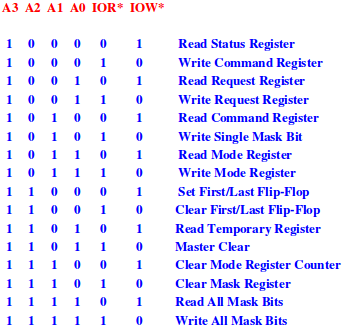
\includegraphics[width=.5\textwidth]{images/letturaregistridmac.png}
%   \caption{Configurazione dei segnali in ingresso al DMAC per la
%     lettura dei registri}
%   \label{letturaregistridmac}
% \end{figure}

% \begin{figure}[h]
%   \centering
%   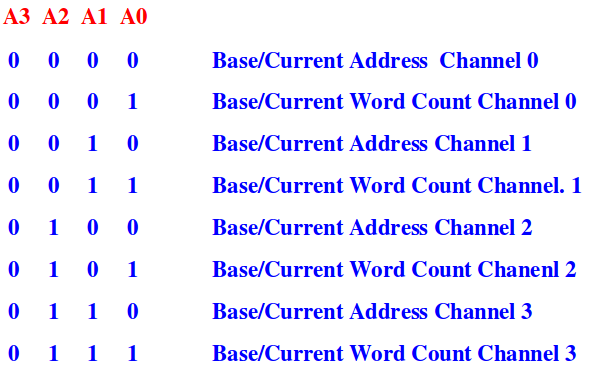
\includegraphics[width=.5\textwidth]{images/letturaregistridmac2.png}
%   \caption{Configurazione dei segnali in ingresso al DMAC per la
%     lettura dei registri}
%   \label{letturaregistridmac2}
% \end{figure}


\section{Fase di trasferimento di dati}

Mentre quando viene programmato il DMAC \`e slave, quando prende il
controllo del canale ed effettua le operazioni di trasferimento dati
assume il ruolo di \textbf{master}.

Come gi\`a anticipato, in questa fase il DMAC attiva il segnale
\texttt{HOLD} e rimane in tale stato finch\'e non riceve il segnale
\texttt{HOLDA} dalla CPU. A questo punto presenta sui piedini
\texttt{D[7..0]} i bit dall'8 al 16 dell'indirizzo di memoria ed
attiva il segnale \texttt{ADSTB} per la sua memorizzazione in un latch
esterno. Invia inoltre su {\tt A[7..0} gli 8 bit meno significativi
dell'indirizzo. Viene attivata successivamente l'uscita \texttt{AEN}
che abilita la lettura della parte d'indirizzo memorizzata nel
latch. Si abilita il segnale \texttt{DACKi} corrispondente al canale
\textit{i} che ha effettuata la richiesta con \texttt{DREQi}. Si
attiva la coppia di segnali di lettura da memoria e scrittura su
periferica o di lettura da periferica e scrittura su memoria.

\section{Generare indirizzi a 32 bit}

Sappiamo che il DMAC 8237 era inizialmente in grado di generare
indirizzi utilizzando solo 8 bit e che \`e stato poi esteso per
generare indirizzi a 16 bit. Tuttavia questo ancora non basta. Ora
abbiamo bisogno di indirizzi a 32 bit. Come possiamo fare? Per ogni
canale del DMA controller \textbf{aggiungiamo due latch da 8 bit}
come mostrato in figura \ref{estensionelatch}.

\begin{figure}[h]
  \centering
  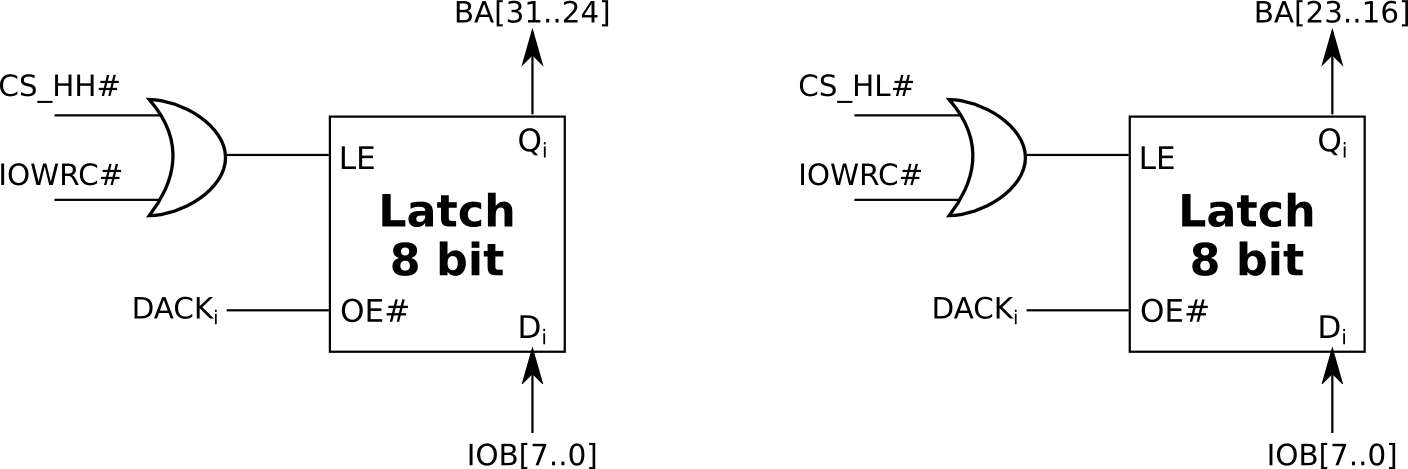
\includegraphics[width=.8\textwidth]{images/estensionelatch.png}
  \caption{Latch 8-bit per generare la parte alta dell'indirizzo}
  \label{estensionelatch}
\end{figure}

In questa configurazione solo la CPU pu\`o modificare i latch pertanto
questi due latch realizzano l'estensione del registro \texttt{BAR} che
non \`e modificabile e non del {\tt CAR} che invece viene aggiornato
ad ogni trasferimento elementare.

Se \`e possibile facilmente estendere i registri \texttt{BAR}, lo
stesso non si pu\`o dire di \texttt{CCR} e \texttt{BCR} che rimangono
a 16 bit; rimante pertanto la limitazione a 64 K per la quantit\`a di
dati trasferibili in una transazione ($2^{16} = 64 K$).

Una possibile alternativa al modello presentato \`e quella di
utilizzare un'unica coppia di latch e non una per ogni canale. In
questo caso i latch verrebbero abilitati dal segnale \texttt{HOLDA}
che corrisponde all'\texttt{OR} fra i quattro segnali \texttt{DACKi}.

\

\textbf{TODO:} cosa succede se voglio trasferire finestre a cavallo
fra due pagine di 64K allineate? Slide 16 di \textit{Interfacciamento
  DMAC}.

\

Vediamo ora come si possa realizzare l'indirizzamento byte per byte di
aree di memoria contigue. Abbiamo bisogno di generare indirizzi a 32
bit. Vediamo come vengono generati tali indirizzi.

Iniziamo vedendo come vengano generati i segnali di \textbf{Bank
  Enable}. Abbiamo a che fare con 8 segnali \texttt{BE0\#..BE7\#},
quindi si utilizzano i 3 bit meno significativi \texttt{A[2..0]} per
generarli. Dai pin \texttt{A[2..0]} devono quindi partire dei segnali
che entrino in un \textbf{decoder 3-8}. L'uscita di questi decoder \`e
abilitata tramite un driver pilotato dal segnale \texttt{HOLDA} e
quindi solo quando il DMAC \`e master. Quando il DMAC \`e slave
dev'essere attivo il percorso inverso perch\'e tramite il Bank Enable
(dopo averlo fatto passare per un \textbf{Encoder 8-3} ed averne
abilitato l'uscita con un altro driver) si devono generare 3 dei 4 bit
che selezionano il registro del DMAC da leggere/scrivere. Si perviene
pertanto ad una struttura come quella riportata in figura
\ref{latchdestra}.

\begin{figure}[h]
  \centering
  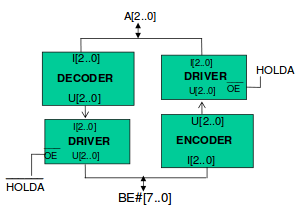
\includegraphics[width=.4\textwidth]{images/latchdestra.png}
  \label{latchdestra}
  \caption{Da \texttt{BE0\#..BE7\#} a \texttt{A[2..0]} e viceversa}
\end{figure}

Il bit \texttt{BA3} dell'indirizzo viene generato dal DMAC tramite il
piedino \texttt{A3} quando questo \`e master, ma nel momento in cui
\`e slave diventa un ingresso proveniente dal bus degli indirizzi e
volto a formare con \texttt{A[2..0]} i bit che selezionano i registri
del DMAC da leggere/scrivere. Ecco dunque la necessit\`a di un
\textbf{tranceiver} che determini il verso di percorrenza del tratto
da \texttt{A3} al bit \texttt{BA3} del bus degli indirizzi. Segue la
struttura di figura \ref{a3ba3}.

\begin{figure}[h]
  \centering
  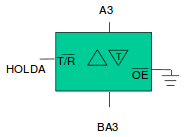
\includegraphics[width=.25\textwidth]{images/a3ba3.png}
  \label{a3ba3}
  \caption{Da \texttt{BA3} ad \texttt{A3} e viceversa}
\end{figure}

Ora \`e la volta dei bit \texttt{A[7..4]}. Questi bit servono soltanto
nel momento in cui il DMAC \`e master in quanto deve generare gli
indirizzi. Quando \`e slave non vengono utilizzati. Anche qui
utlizziamo perci\`o un \textbf{driver} comandato da \texttt{HOLDA}.

\begin{figure}[h]
  \centering
  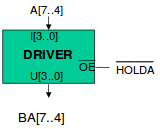
\includegraphics[width=.25\textwidth]{images/a74.png}
  \label{a74}
  \caption{Da \texttt{A[7..4]} a \texttt{BA[7..4]}}
\end{figure}

\section{Riferimenti}

\subsection{Libri}
\begin{itemize}
\item \textbf{Architettura ed organizzazione dei calcolatori
    elettronici} di \textit{Giacomo Bucci}
\end{itemize}

\subsection{Link}
\begin{itemize}
\item \url{http://www.cast-inc.com/ip-cores/dmas/c8237/cast_c8237-a.pdf}
\end{itemize}

\end{document}